\documentclass[11pt]{article}

\usepackage[a4paper,margin=1in]{geometry}
\usepackage{graphicx}
\usepackage{xcolor}
\usepackage{enumitem}
\usepackage{hyperref}
\usepackage{caption}
\usepackage[numbers,sort&compress]{natbib}

\hypersetup{
  colorlinks=true,
  linkcolor=black,
  citecolor=black,
  urlcolor=black
}

\setlength{\parindent}{0pt}
\setlength{\parskip}{0.65em}
\setlist[itemize]{leftmargin=1.4em,itemsep=0.25em,topsep=0.25em}
\setlist[enumerate]{leftmargin=1.5em,itemsep=0.25em,topsep=0.25em}

\newcommand{\journal}{\textit{Nature Reviews Earth \& Environment}}
\newcommand{\papertitle}{From greenness to function in ecosystem monitoring}

\begin{document}

\begin{center}
{\Large \textbf{Presubmission inquiry}}\\[0.25em]
{\large \journal}\\[0.45em]
{\large \textbf{\papertitle}}
\end{center}

Dear Editors,

We would like to ask whether the proposed Perspective, \textbf{``\papertitle''}, would be of interest to \journal.

Operational ecosystem monitoring has become increasingly continuous in space and time, but much of its ecological interpretation still rests on greenness and broad structural proxies. These variables are indispensable, yet they often conflate pigment dynamics, canopy state, water limitation, phenology, disturbance history and viewing geometry. At the same time, spaceborne imaging spectroscopy is entering a new phase through PRISMA, EnMAP, EMIT and forthcoming CHIME/SBG-class missions, while Landsat and Sentinel-2 provide dense temporal archives. We argue that the next step is to move from spectral snapshots to functional ecosystem monitoring: continuous, uncertainty-aware functional observables that are anchored by imaging spectroscopy, reconstructed through time with dense multispectral records and interpreted using explicit ecological guardrails.

The manuscript is not a literature review of hyperspectral remote sensing and is not a case-study paper. It is a forward-looking Perspective that defines what would make trait-enabled ecosystem monitoring scientifically credible. Its central contribution is a measurement framework that distinguishes traits that are directly or strongly anchored by spectroscopy from traits that are inferred through trait covariation, temporal context, canopy state and ecological correlation. It also makes explicit that canopy structure should be constrained by complementary observations such as LiDAR, SAR and InSAR rather than implied as a direct hyperspectral product.

We develop four main ideas:

\begin{enumerate}
\item ecosystem monitoring needs functional observables that go beyond greenness anomalies;
\item imaging spectroscopy is best framed as a trait-anchor system, while multispectral archives provide temporal continuity and LiDAR/SAR/InSAR constrain structural state;
\item continuous functional observables could support stress-syndrome attribution, resistance, recovery, legacy-effect analysis, dynamic functional diversity and Earth-system model evaluation;
\item operational products need a reporting contract, including trait definitions, uncertainty calibration, provenance, domain-of-applicability masks and validation across sites, years and ecological contexts.
\end{enumerate}

An early European forest proof-of-concept is included only to show that the sparse-to-dense framework is technically implementable with current Earth observation archives. It is presented as an illustration, not as a complete benchmark or as the main claim of the manuscript. The broader argument is global and conceptual.

We believe this article would be timely for \journal\ because the field is approaching a transition from mission-driven spectral data products to ecology-facing functional monitoring products. The article would speak to remote sensing scientists, ecologists, Earth-system modellers and environmental monitoring communities.

The planned article length is approximately 4,000--4,500 words, with five display items:

\begin{enumerate}
\item the conceptual shift from greenness proxies to functional observables;
\item a complementary-observation framework linking imaging spectroscopy, LiDAR/SAR/InSAR and dense multispectral archives;
\item a compact European forest proof-of-concept;
\item trait anomalies for stress, resistance, recovery and legacy effects;
\item a roadmap and reporting contract for credible functional ecosystem monitoring.
\end{enumerate}

We would be grateful for your advice on whether this proposed Perspective fits the scope and commissioning priorities of the journal.

Sincerely,

Chaonan Ji, on behalf of the co-authors

\clearpage
\section*{Optional supporting note}

This page is intended as supporting material for the presubmission inquiry, not as a full manuscript submission.

\textbf{Article type and positioning.}
The proposed article is a Perspective. It uses an early European forest analysis only as proof-of-concept, while the main contribution is a conceptual and operational framework for continuous functional observables.

\textbf{Why the topic is timely.}
The timing is driven by three converging developments: spaceborne imaging spectroscopy from PRISMA, EnMAP and EMIT, forthcoming CHIME/SBG-class mission concepts, and dense multispectral archives that can provide temporal continuity. Recent trait-spectroscopy studies show increasing maturity in transferable multi-trait retrieval and spectral-trait databases \citep{cherif2023spectra,mederer2025plant,wu2026gsti,ji2024transferability,ji2025transferlearning,ji2025prisma}, while ecological monitoring still needs interpretable variables for stress, recovery, legacy effects and model evaluation \citep{pettorelli2018satellite,zeng2022optical,cavender2025spectral}.

\textbf{Core boundary condition.}
The manuscript explicitly avoids treating hyperspectral imagery as a direct source of detailed canopy structure. Imaging spectroscopy is framed as a biochemical and optical trait-anchor system; structural variables should be constrained with LiDAR, SAR and InSAR where needed \citep{dubayah2024structural,lang2024gedi}.

\textbf{Main novelty.}
The novelty is not another review of hyperspectral retrieval methods. The article argues for a measurement contract that turns sparse spectral trait anchors into continuous functional monitoring variables with uncertainty, provenance, domain-of-applicability masks and ecological validation.

\section*{Display-item preview}

The full manuscript package contains current draft figures. Figure 1 is still intended for redesign; Figures 2--5 are reproducible generated figures.

\begin{figure}[h]
\centering
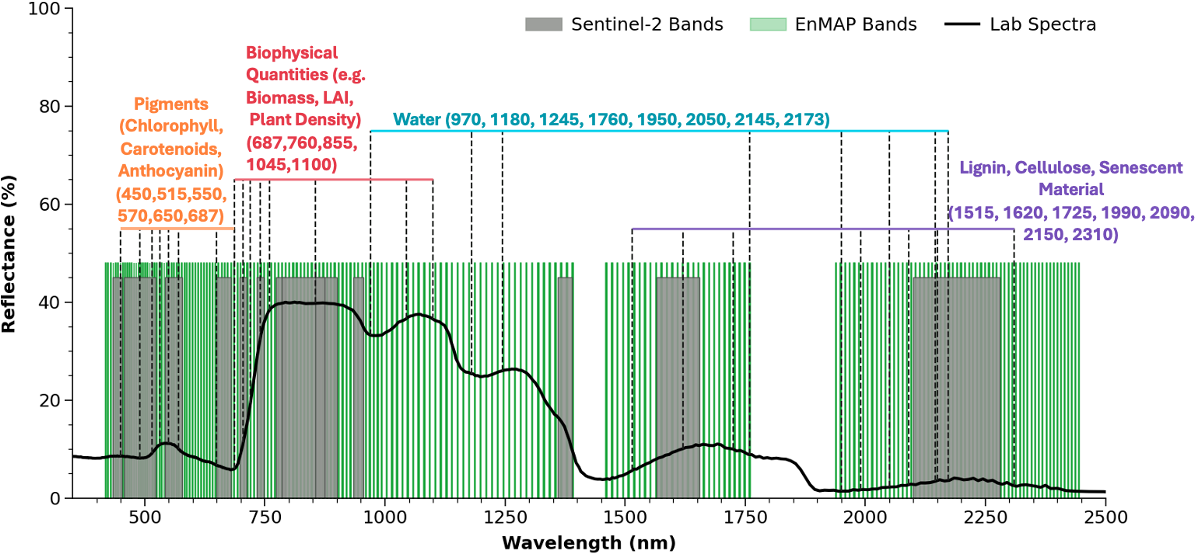
\includegraphics[width=0.86\textwidth]{../figures/draft/fig1_spectra_original.png}
\caption*{\textbf{Display item 1, draft concept.} From spectral information to plant function. This existing concept figure should be redrawn as the flagship visual for the Perspective.}
\end{figure}

\begin{figure}[h]
\centering
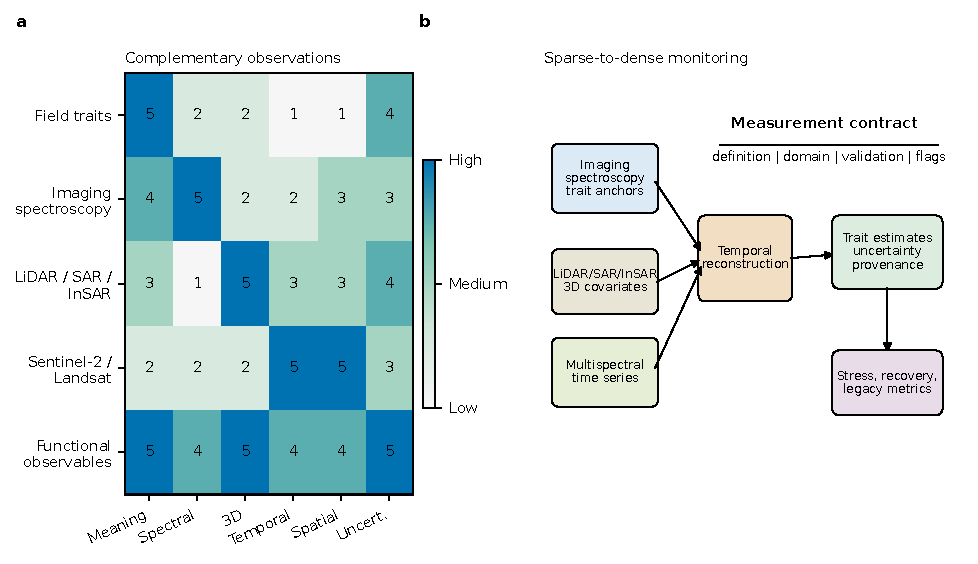
\includegraphics[width=0.96\textwidth]{../figures/generated/fig2_functional_observables_framework.pdf}
\caption*{\textbf{Display item 2.} Complementary observations and sparse-to-dense monitoring framework.}
\end{figure}

\begin{figure}[h]
\centering
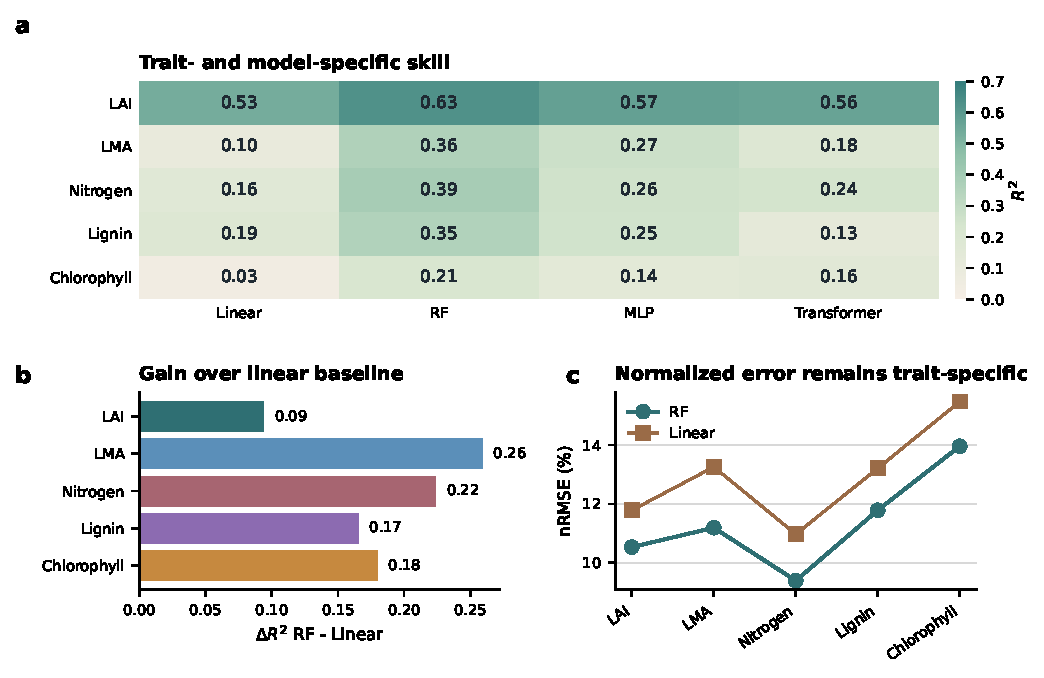
\includegraphics[width=0.96\textwidth]{../figures/generated/fig3_proof_of_concept_performance.pdf}
\caption*{\textbf{Display item 3.} Compact European forest proof-of-concept, interpreted as feasibility evidence rather than an operational benchmark.}
\end{figure}

\begin{figure}[h]
\centering
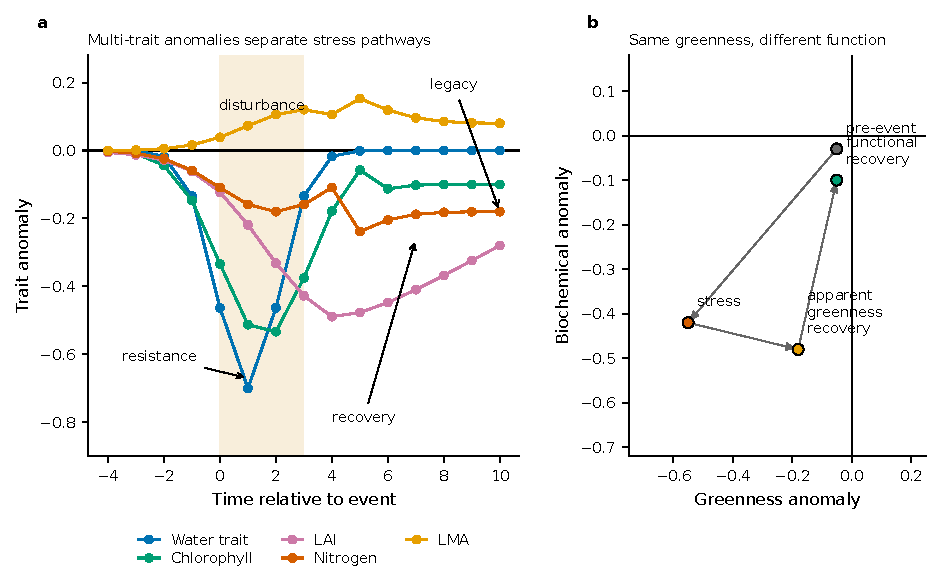
\includegraphics[width=0.96\textwidth]{../figures/generated/fig4_trait_anomaly_syndromes.pdf}
\caption*{\textbf{Display item 4.} Trait anomalies for stress, resistance, recovery and legacy effects.}
\end{figure}

\begin{figure}[h]
\centering
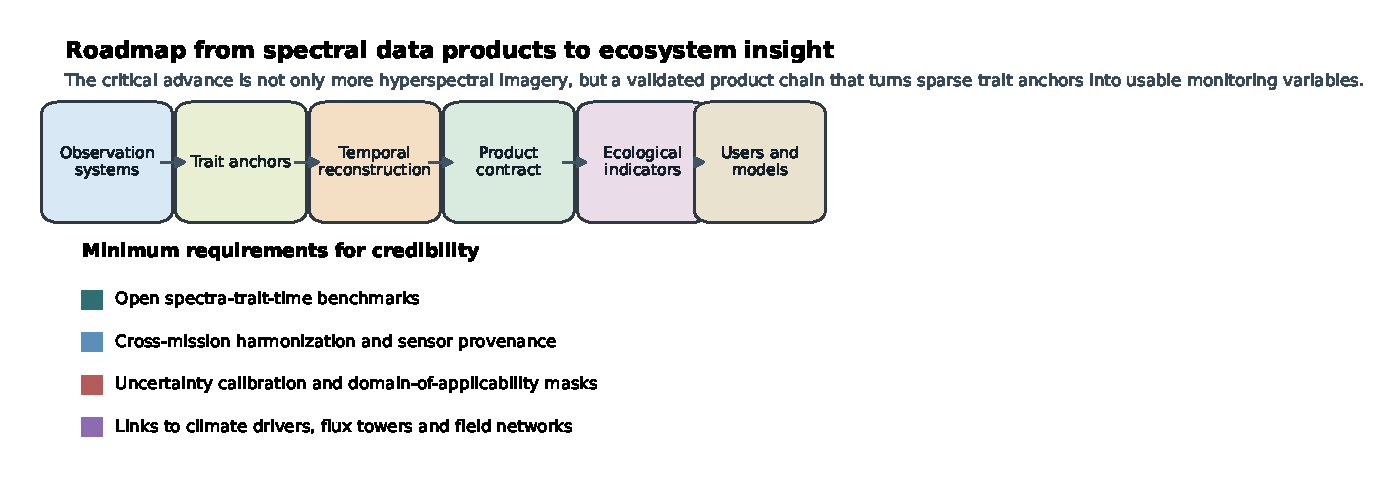
\includegraphics[width=0.96\textwidth]{../figures/generated/fig5_monitoring_roadmap.pdf}
\caption*{\textbf{Display item 5.} Roadmap and minimum requirements for credible functional ecosystem monitoring.}
\end{figure}

\clearpage
\bibliographystyle{unsrtnat}
\bibliography{../references}

\end{document}
